%--
%-- Modelo de Objetivos
%--
\clearpage
\subsection{Modelo de Objetivos}

\subsubsection{Listado de objetivos}

\paragraph{1 - Objetivo primario}

El objetivo primario del sistema es revertir la disminución de ventas (1) que se
viene produciendo en la cadena de supermercados hace meses. Para ello, se nos
brinda la información de que las dos causas de las disminuciones son las largas
colas en el supermercado y el agotamiento del stock (1.3), de donde se
desprenden los objetivos (1.1) y (1.2).

\paragraph{1.1 - Reducción de colas}

Dentro del contexto de la reducción de colas, se tomó la presunción de que cada
venta online estaría disminuyendo las colas en la sucursal (1.1.2), dado que de
este modo ese cliente, que normalmente estaría haciendo cola en el supermercado,
puede encargar los productos desde la comodidad de su casa. De este modo, se
toma el objetivo de permitir que el usuario compre de forma online (1.1.1).

\paragraph{1.1.1 - Permitir al usuario la compra online}

Consideramos que para permitir que el cliente compre un pedido de forma online,
deben ocurrir dos cosas, lograr que el cliente encargue el pedido (1.1.1.1)
\footnote{lo cual incluye todo el proceso desde que el cliente se registra en
el sitio, realizando la selección de productos, acordando una fecha de entrega y
eligiendo una forma de pago}, y lograr que el pedido sea cerrado y finalizado
(1.1.1.2), que comienza con la confirmación del pedido por parte del cliente, y
culmina con la entrega del pedido (o la cancelación/anulación, según el caso).

\paragraph{1.1.1.1 - Lograr[Cliente encarga pedido]}

Para que un cliente encargue un pedido, es necesario que el mismo pueda
identificarse en el sistema (1.1.1.1.1), que el pedido sea armado (1.1.1.1.2),
que se pueda acordar una fecha de entrega (1.1.1.1.3), una forma de pago
(1.1.1.1.4) y que si esta última es online, se le pueda cobrar.

\paragraph{1.1.1.1.1 - Lograr[Cliente identificado]}

Para que el cliente pueda ser identificado por el sistema, es necesario que se
encuentre registrado (1.1.1.1.1.1), y que se autentique (1.1.1.1.1.2)

\paragraph{1.1.1.1.1.1 - Lograr[Cliente registrado]}

La forma en que un cliente se registra es uno de los o-refinamientos
propuestos. Dividimos el registro entre online y presencial. El registro
online implica que el cliente se conecte al sitio, cargando sus datos
personales, y sus datos de pago, los cuales son verificados por el sistema al
momento de la registración. El registro presencial, en cambio, requiere que el
cliente se dirija a la sucursal con la documentación necesaria para verificar
identidad, domicilio y datos de pago, los cuales son archivados y verificados
por un empleado de la sucursal, y posteriormente cargados al sistema. Más
pormenores sobre este refinamiento, junto con la justificación del puntaje
asignado a los objetivos blandos, están explicados posteriormente.

\paragraph{1.1.1.1.1.2 - Lograr[Cliente se autentica de forma segura]}

La autenticación requiere que el cliente ingrese sus credenciales
(1.1.1.1.1.2.1). Por otro lado, también es necesario proveer una interfaz que
cuente con los mecanismos de seguridad adecuados (1.1.1.1.1.2.2), por ejemplo
conexión HTTPS.

\paragraph{1.1.1.1.2 - Lograr[Armado de pedido]}

Para que el pedido sea armado, consideramos que es necesario que el cliente
pueda ver el stock disponible para cada producto (1.1.1.1.2.1), y que logre
seleccionar la mercadería adecuada (1.1.1.1.2.3). Para ello, planteamos el
objetivo de mostrar recomendaciones personalizadas para cada cliente
(1.1.1.1.2.2), que varían según los distintos datos relacionados a su usuario,
como pueden ser, perfil de comprador, generado a través del historial de
compras, compras de otros clientes, relacionados según escala socioeconómica,
edad, domicilio, etc.

\paragraph{1.1.1.1.3 - Lograr[Acordar fecha de entrega]}

En el transcurso del armado del pedido, es necesario que el cliente acuerde una
fecha de entrega. Para ello, es necesario que el sistema le ofrezca un rango de
fechas disponibles (1.1.1.1.3.2), las cuales serán calculadas e informadas por
logística (1.1.1.1.3.1), y obtenidas en tiempo real, de algun modo, por ejemplo
a través de algún tipo de interfaz entre nuestro sistema y el sistema de
logística. En caso de no haberla, será necesario contar con una forma de
calcularla. Luego de mostrarles las fechas, el cliente eligirá (1.1.1.1.3.3) la
que más le convenga.

\paragraph{1.1.1.1.4 - Lograr[Acordar forma de pago]}

Además de que el cliente seleccione la fecha de entrega, es necesario que
acuerde con el sistema una forma de pago. Para ello, el sistema deberá informar
al cliente cuales son las formas de pago que tiene disponibles (1.1.1.1.4.2), y
el cliente deberá elegir entonces la que le resulte de su conveniencia
(1.1.1.1.4.3). Hay un o-refinamiento aquí, sobre el objetivo de evaluar si se
deberá permitir la contraentrega.

\paragraph{1.1.1.1.4.1 - Lograr[Evaluar si permitir contraentrega]}

Para evaluar si el cliente puede realizar un pedido por contrareembolso,
proponemos dos opciones. La primera de ellas, es un límite de entregas fallidas,
contenido dentro de la programación del sistema, e instanciado en 1 en nuestros
ejemplos, es decir, se limita la posibilidad de que el cliente .

\fixme[RETOMAR ESTA EXPLICACIÓN]

\paragraph{1.1.1.1.5 - Lograr[Si la forma de pago es online, cobrar]}

Si el cliente elige el pago online, además, hay que cobrarle. Para ello, se
cuenta con la participación del cliente, el cual deberá validarse a través del
agente de cobro, para que el importe le sea deducido de su cuenta bancaria.

\paragraph{1.1.1.2 - Lograr[El pedido es finalizado y cerrado]}

Una vez que un pedido está encargado, es necesario que el mismo sea cerrado.
Aquí pueden ocurrir dos cosas, que el usuario cancele el pedido antes de que el
mismo sea preparado (1.1.1.2.2), caso en el que el mismo se anula y se le
devuelve el dinero, o que el usuario confirme el pedido (1.1.1.2.1). En este
último caso, será necesario preparar el pedido (1.1.1.2.1.1) a la vez que el
stock es restado del conteo del sistema (1.1.1.2.1.2), y luego lograr que el
mismo sea entregado a logística (1.1.1.2.1.3). Además de todo esto, será
necesario asegurar que el envío sea realizado (1.1.1.2.1.4).

\paragraph{1.1.1.2.1.4 - Lograr[Realizar el envío]}

Al momento de realizar el envío, pueden ocurrir dos situaciones, o que el
cliente reciba el pedido (1.1.1.2.1.4.1), o que no lo reciba (1.1.1.2.1.4.2).
Por simplicidad, se englobaron todas las situaciones en las que el cliente puede
no recibir el pedido, en una situación ``el cliente no está presente''. Es
decir, también es este el caso cuando un cliente esta presente pero por alguna
razón se niega a recibir el pedido.

\paragraph{1.1.1.2.1.4.2 - Lograr[Realizar el envío]}

En caso de que el cliente no reciba el pedido, será necesario deshacer la
operación, es decir, reintegrar el dinero de ser necesario (1.1.1.2.1.4.2.1),
marcar el pedido como no recibido en el historial del cliente (1.1.1.2.1.4.2.2),
y que logística devuelva el stock al depósito para que sea reingresado
(1.1.1.2.1.4.2.3). Esto significa que Depósito realizará la evaluación de los
productos (ya que algunos pueden haberse roto o perdido su calidad en el
transcurso del envío), y reingresará a stock los que considera que se encuentran
adecuados. Además, se le informará al cliente que su pedido no fue recibido
mediante un email, y se le ofrecerá rehacerlo (1.1.1.2.1.4.2.4).

%--
%-- Modelo de objetivos - Diagramas
%--
\subsubsection{Diagramas de Objetivos}
\begin{figure}[H]
  \begin{center}
  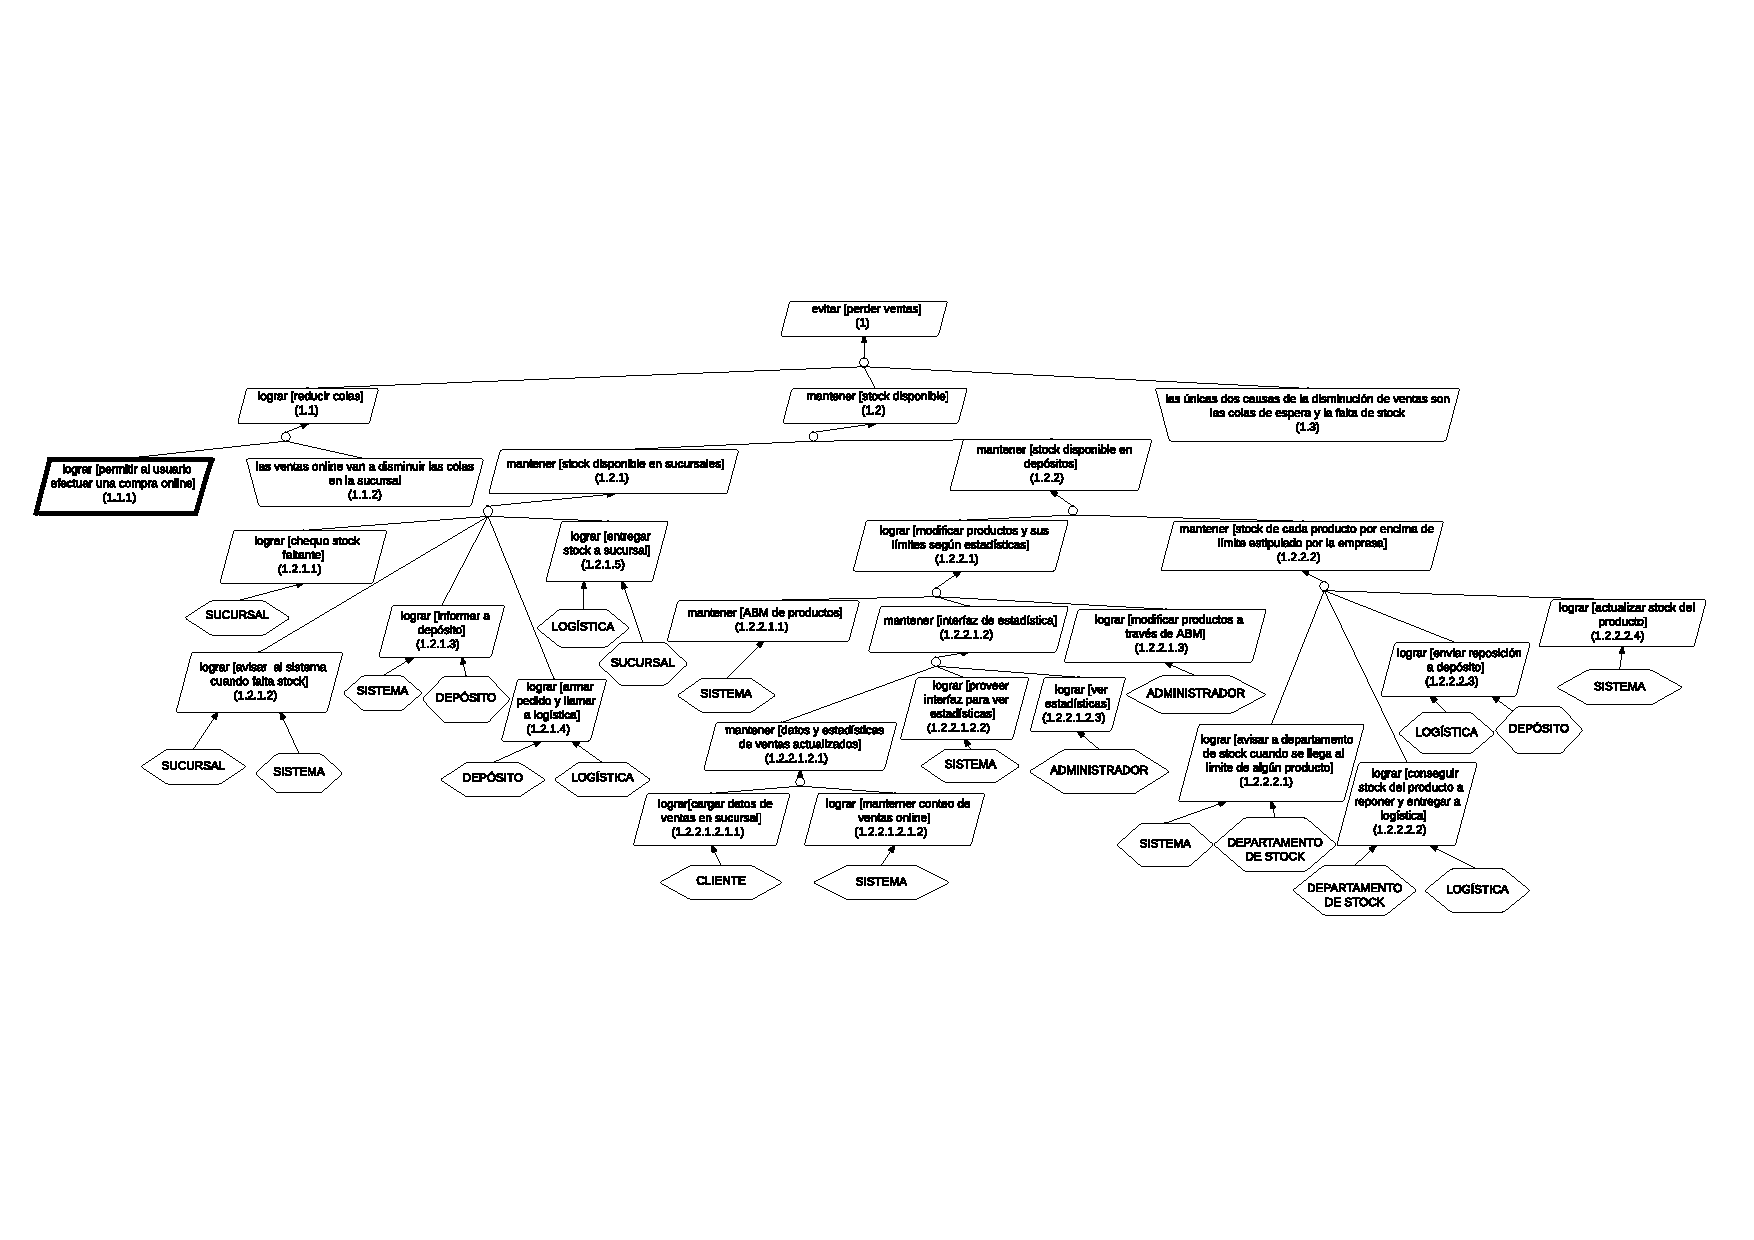
\includegraphics[angle=90,height=\textheight]{images/objetivos-raiz.pdf}
  \caption{Objetivo: Evitar perder ventas}
  \end{center}
\end{figure}

\newpage
\begin{figure}[H]
  \begin{center}
  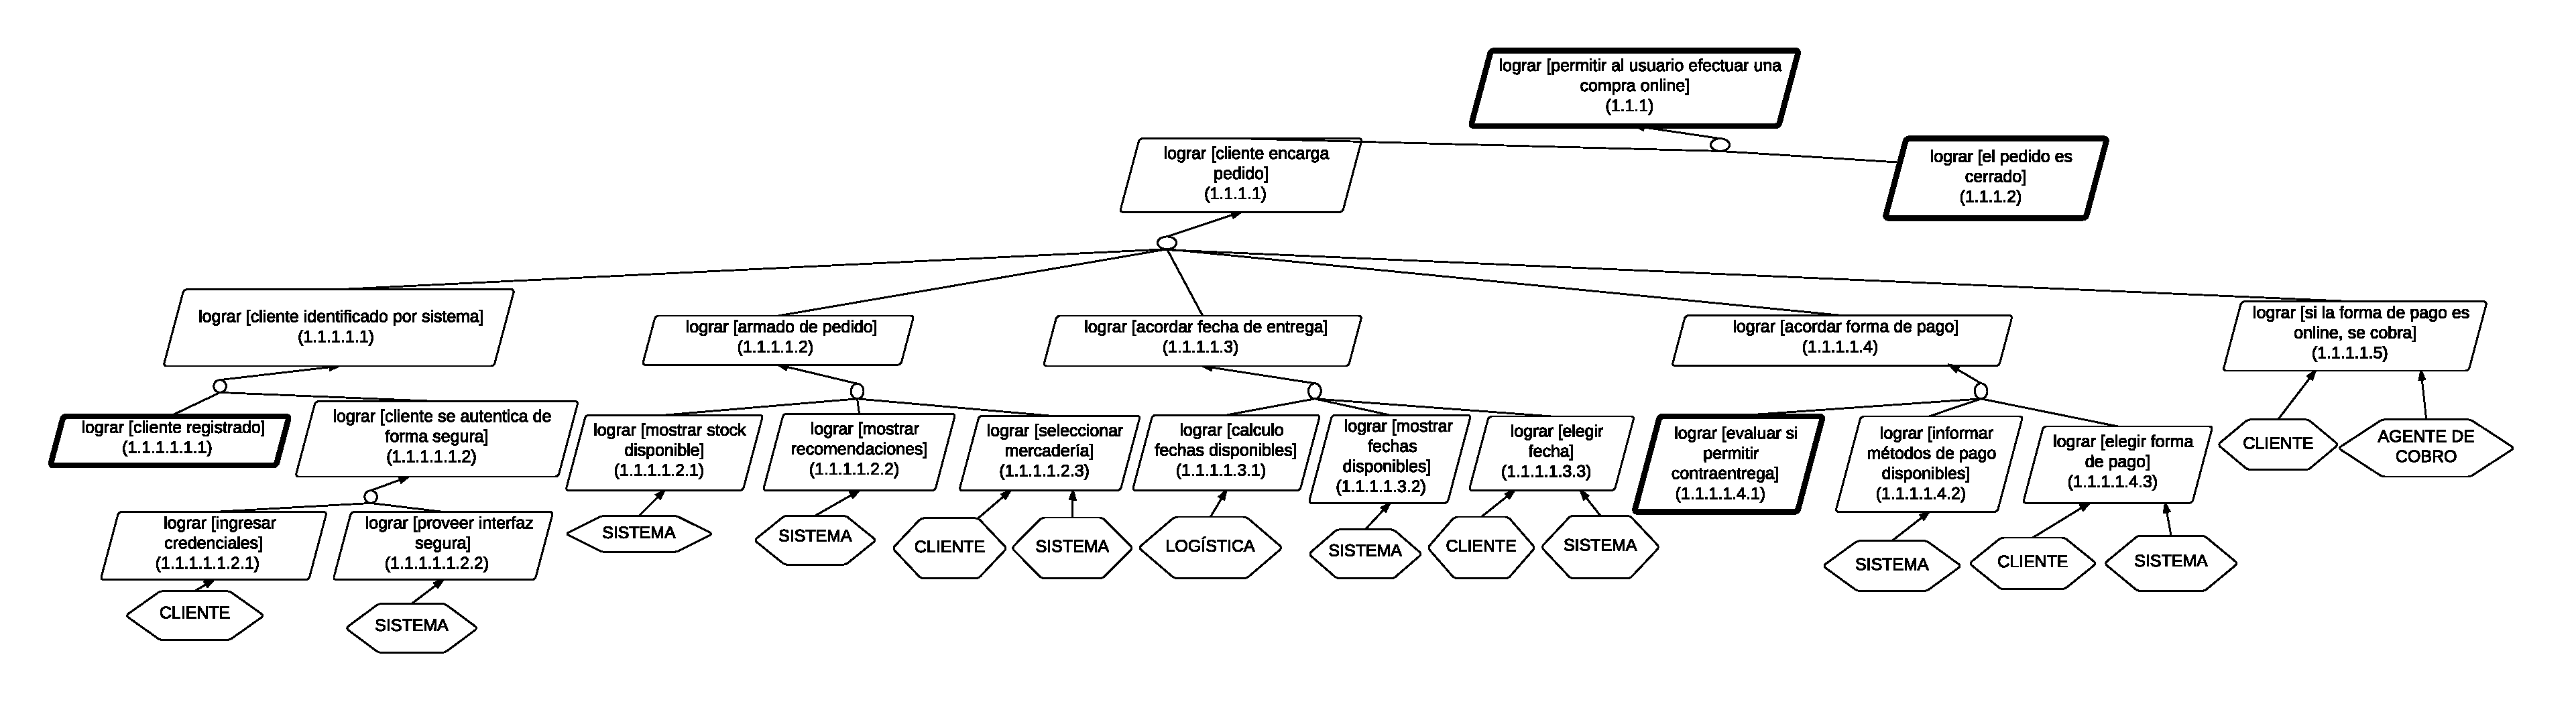
\includegraphics[angle=90,height=\textheight]{images/objetivos-operacion-online.pdf}
  \caption{Objetivo: Lograr permitir al usuario efectuar una compra online}
  \end{center}
\end{figure}

\newpage
\begin{figure}[H]
  \begin{center}
  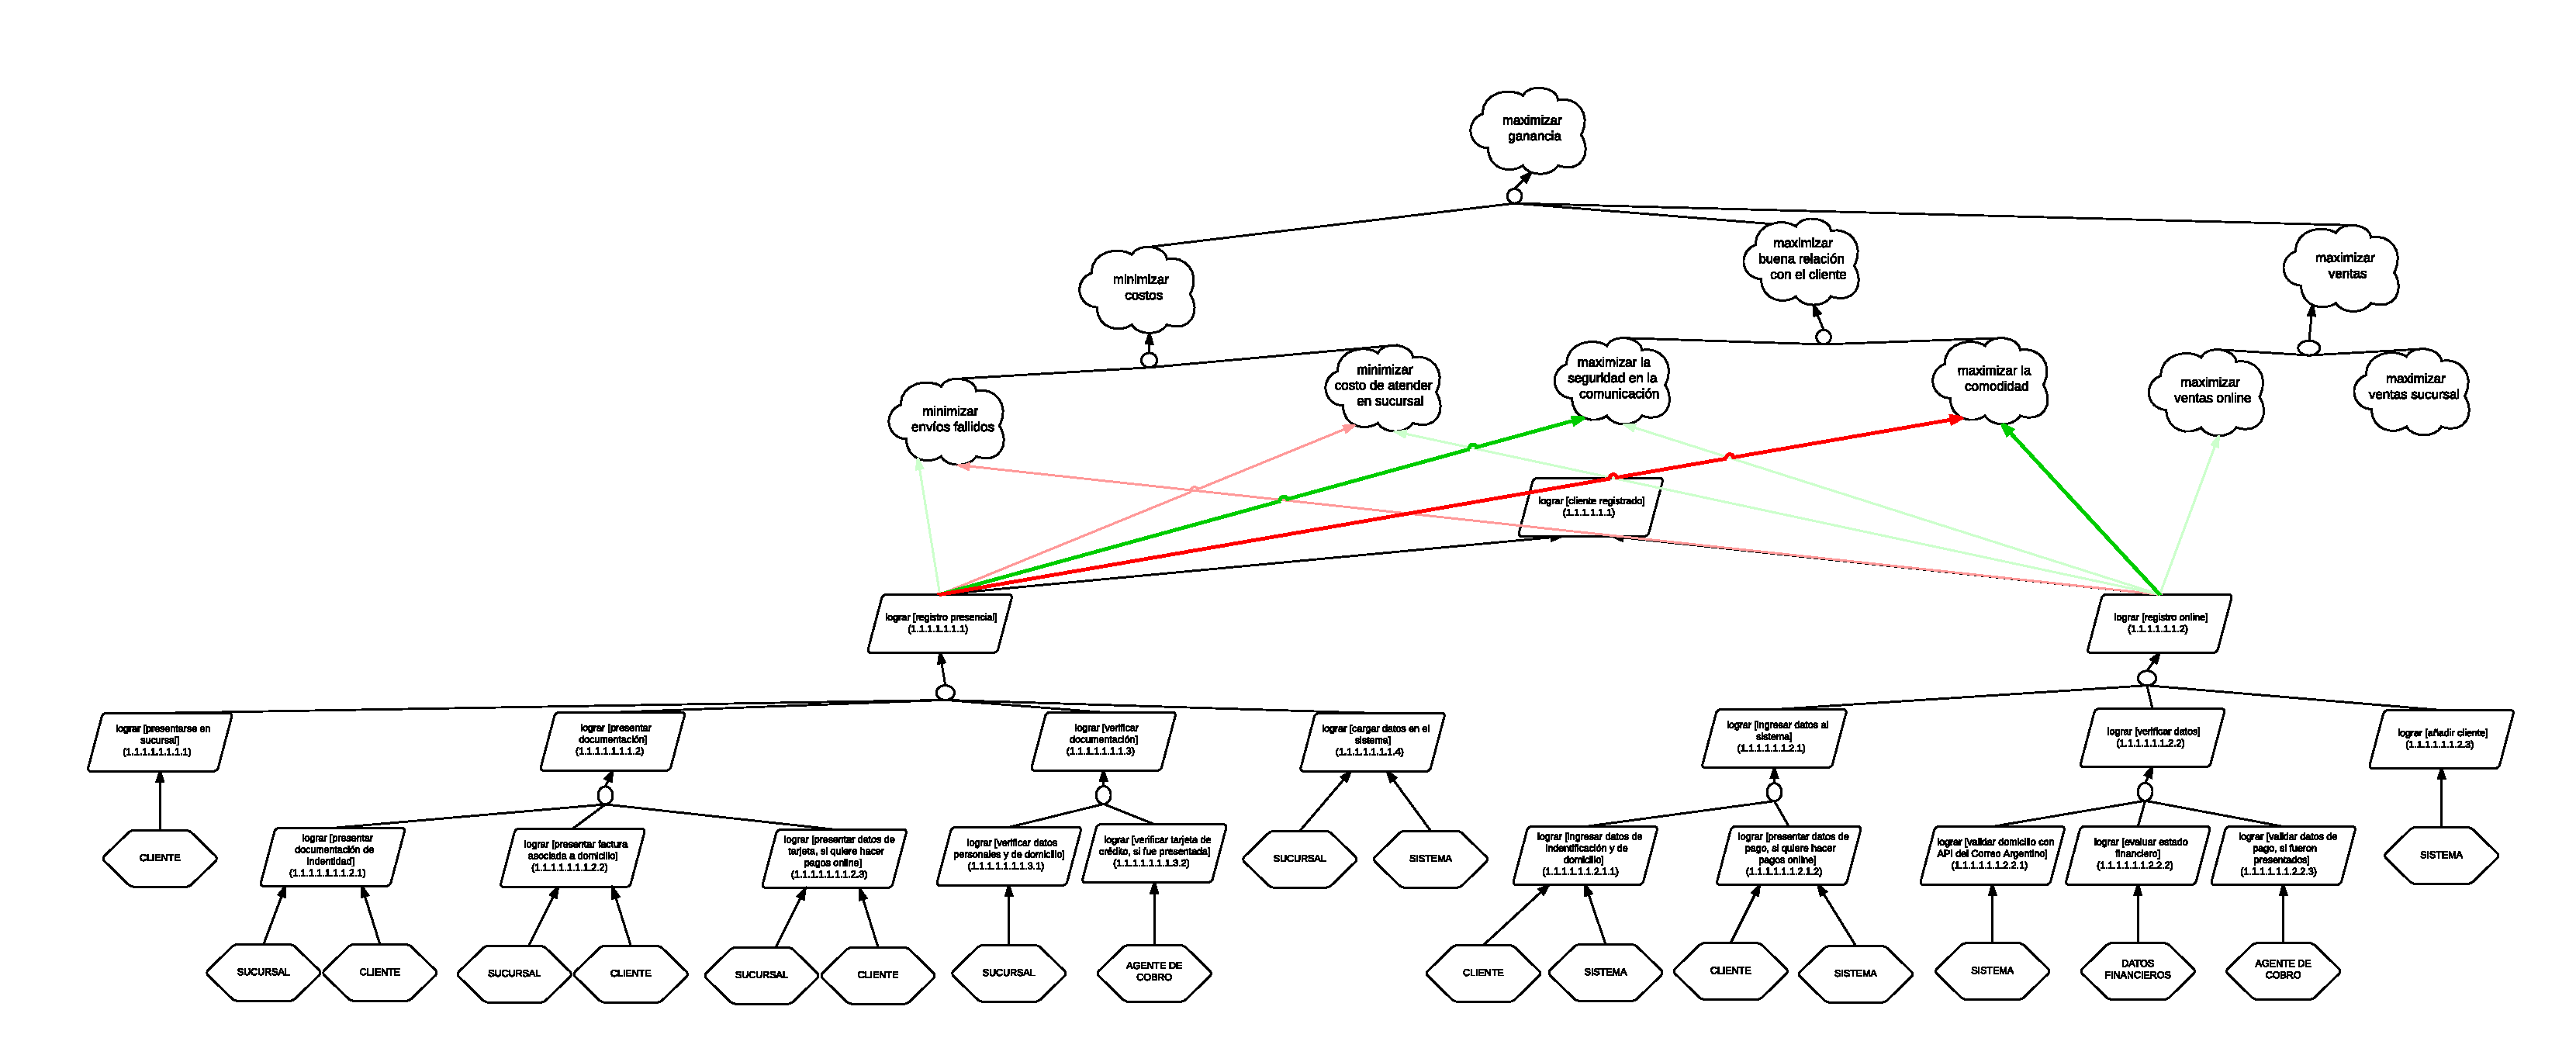
\includegraphics[angle=90,height=\textheight]{images/objetivos-cliente-registrado.pdf}
  \caption{Objetivo: Lograr cliente registrado}
  \end{center}
\end{figure}

\newpage
\begin{figure}[H]
  \begin{center}
  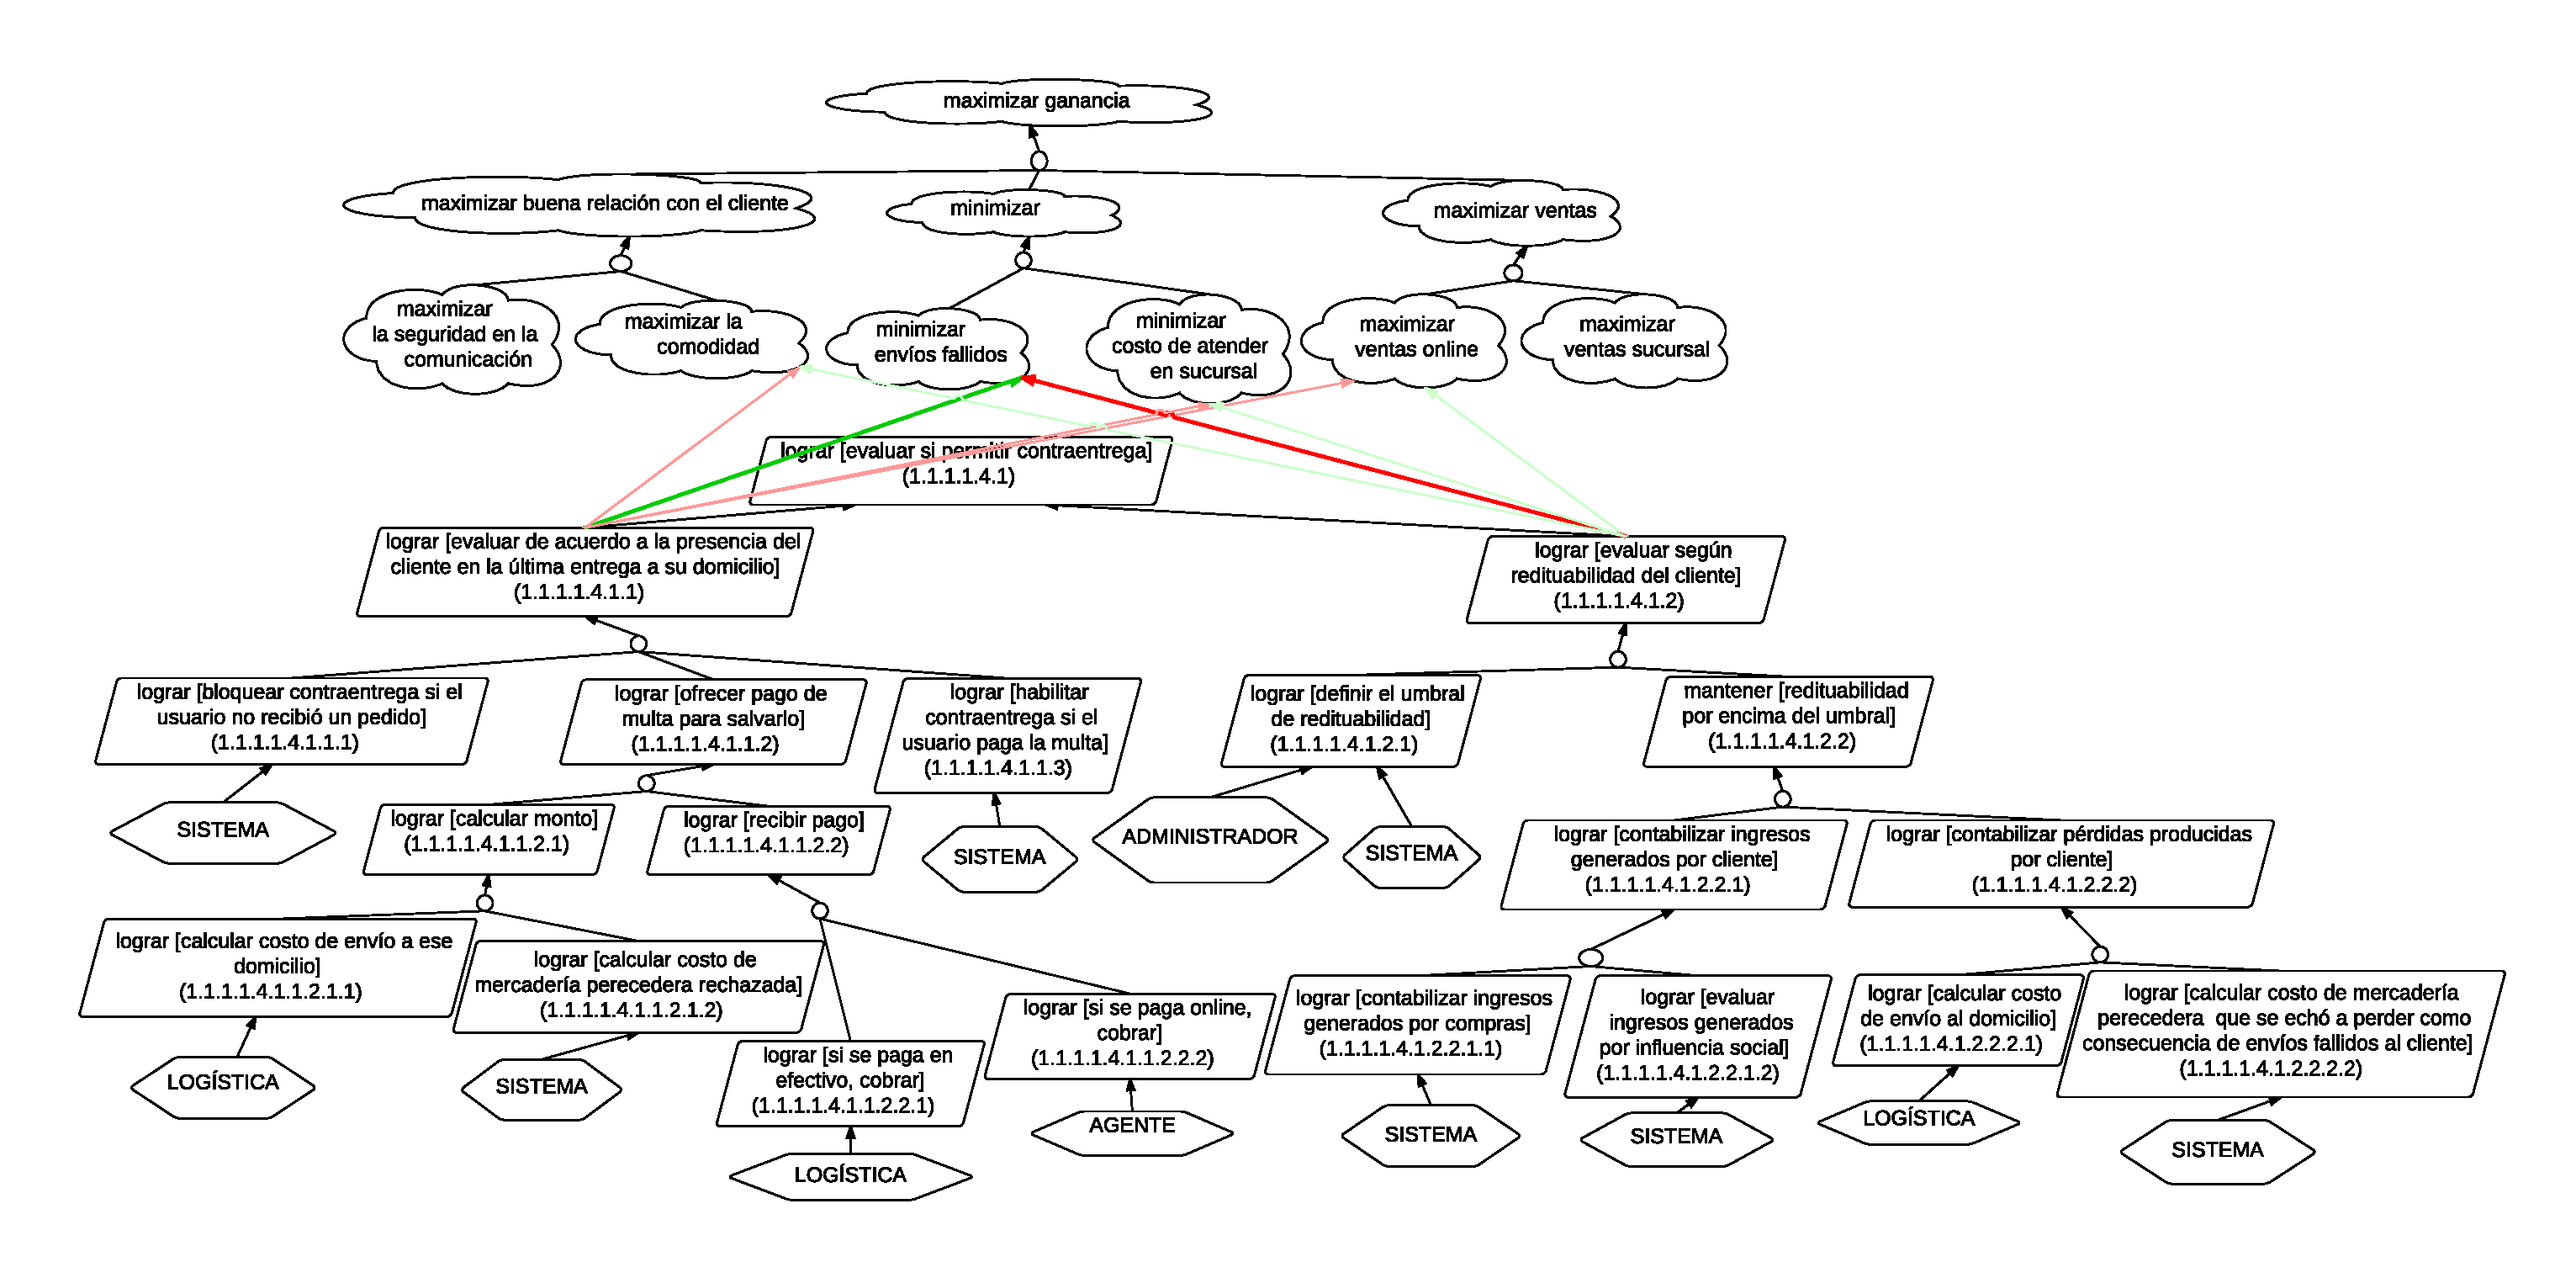
\includegraphics[angle=90,height=\textheight]{images/objetivos-permitir-contraentrega.pdf}
  \caption{Objetivo: Lograr evaluar si permitir contraentrega}
  \end{center}
\end{figure}

\newpage
\begin{figure}[H]
  \begin{center}
  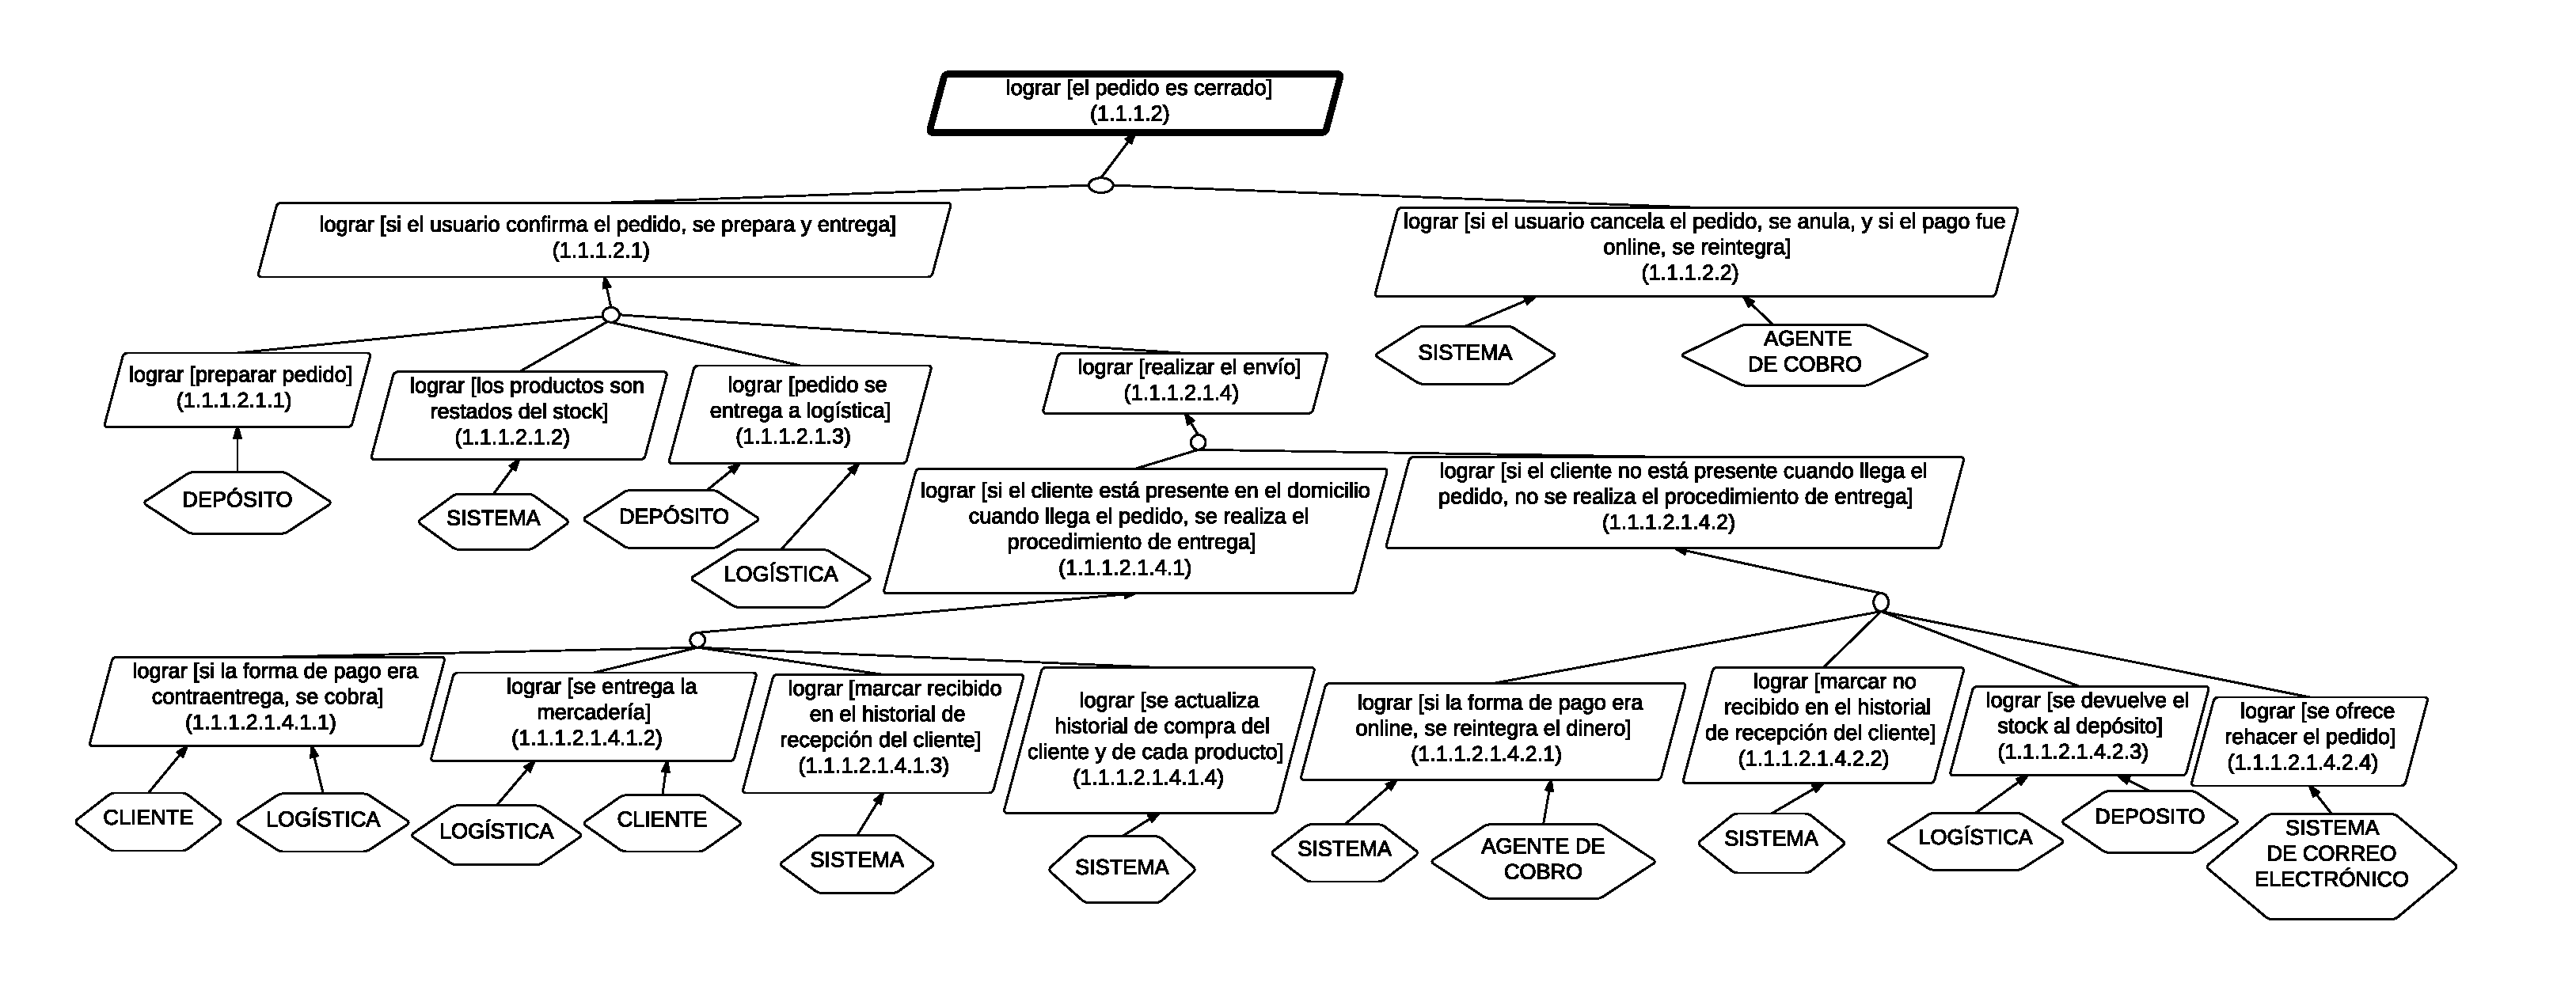
\includegraphics[angle=90,height=\textheight]{images/objetivos-cerrar-pedido.pdf}
  \caption{Objetivo: Lograr el pedido es cerrado}
  \end{center}
\end{figure}

\newpage
\subsubsection{O-Refinamiento: Registro del cliente}
\begin{figure}[H]
  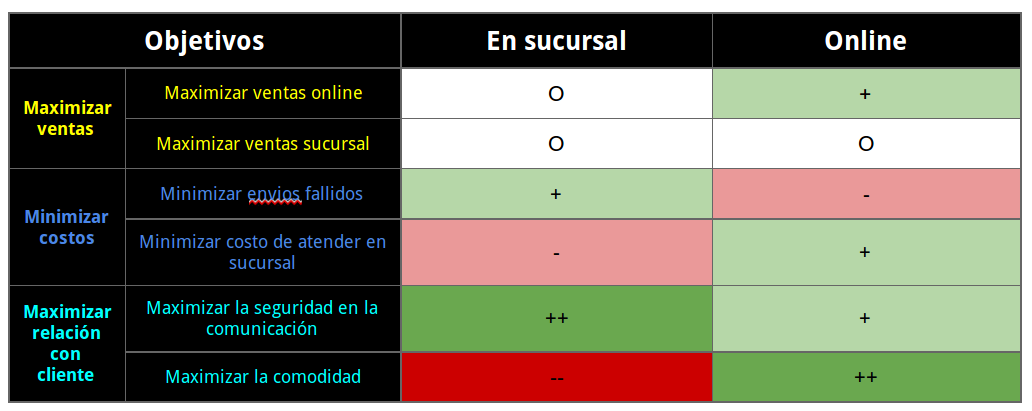
\includegraphics[width=\linewidth]{images/objetivo-blando-registro-cliente.png}
\end{figure}

\paragraph{Ventas}

La opción de registro online es evidentemente más simple y accesible, lo que
ocasionaría que más clientes opten por registrarse y comprar online, sobre todo
aquellos clientes que no acostumbran a comprar normalmente en ese supermercado
(ya que esto no impactaría tanto en los clientes habituales). De lo anterior, se
deduce que la opción de registro online impactaría positivamente en el objetivo
de maximizar las ventas online.

\paragraph{Costos}

Al obligar a los clientes a registrarse presencialmente en una sucursal,
exigiendoles la documentación correspondiente (por ejemplo, dni, un impuesto,
una factura de servicio) que acredite su domicilio y su identidad, se estaría
obteniendo una verificación confiable de los mismos, lo que repercute en una
minimización de los envíos fallidos ocasionados por personas que presentan datos
falsos, o sin ser esta su intención, cometen errores al escribir los datos. El
registro online, por el contrario, aumenta la posibilidad de que sucedan esos
inconvenientes, lo que impactaría negativamente en la minimización de los envíos
fallidos.

\paragraph{Relación con cliente}

\subparagraph{Maximizar la seguridad en la comunicación:}

Al registrar los datos del cliente en la sucursal, en persona, se presume que la
transmisión de los datos del cliente es siempre más segura que si se lo hace
online. De todos modos, según lo solicitado por el CEO, la comunicación se
establecería por un canal seguro, así que el riesgo de robo de información por
medio de una escucha de red se encuentra notablemente suprimido. Desde esa
perspectiva, ambos canales de comunicación tienen un nivel de confiabilidad
similar.

Por otro lado, mediante el canal de registro online, una persona podría llegar a
realizar un registro fraudulento, suplantando la identidad de otra persona,
escudada en el anonimato que ofrece internet, mientras que presencialmente es
mucho más difícil realizar este tipo de prácticas, de lo que concluimos que, si
bien ambos canales son seguros, la vía presencial resulta bastante más
confiable.

\subparagraph{Maximizar la comodidad:}

Obligar al cliente a realizar el registro presencialmente, suponiendo además que
este deba recolectar y presentar toda la documentación pertinente, le puede
llegar a resultar molesto e incómodo. En el peor caso el cliente tendría que
juntar y fotocopiar toda la documentación exigida, dirigirse a una sucursal en
horario laboral, no necesariamente cerca de su domicilio, esperar a ser
atendido, completar algún tipo de formulario, entregar la documentación, y
esperar a que le informen de algún modo que su usuario fue dado de alta.
Mediante el registro online, en cambio, el cliente podrá ingresar al website
desde la comodidad de su casa, en cualquier horario, e ingresar sus datos.
Inmediatamente, entonces, el cliente tendría la posibilidad de realizar una
compra.

\newpage
\subsubsection{O-Refinamiento: Ranking del cliente}
\begin{figure}[H]
  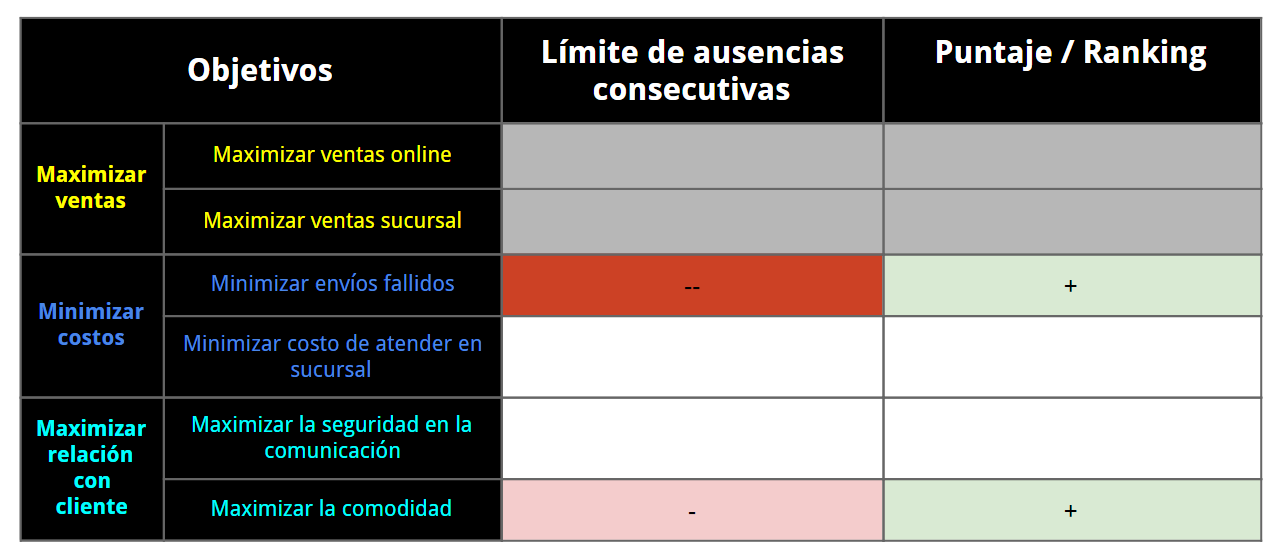
\includegraphics[width=\linewidth]{images/objetivo-blando-ranking-cliente.png}
\end{figure}

\subparagraph{Cliente Bueno / Cliente Malo:}

Llamaremos cliente bueno a aquel que se asume que en el futuro va a producir
ingresos mediante compras de algún tipo. En particular, cuando estemos
hablando de compras online, un cliente bueno será aquel que en el futuro
realizará compras online. Lo mismo sucede con las compras en sucursal. De
igual modo, se define un cliente malo como aquel que, por cualquiera de las
posibles razones, no va generar ingresos (o peor, va a generar costos) en el
futuro. Obviamente, como se está hablando de eventos futuros, siempre que
hablemos de ``clientes buenos'' y ``clientes malos'', se estará hablando de la
posibilidad de que un cliente sea bueno, o de que un cliente sea malo, y no de
una certeza.

\paragraph{Maximizar Ventas:}

\subparagraph{Maximizar Ventas Online:}

Al bloquearle al cliente la posibilidad de realizar ventas online
contrareembolso, si bien es posible que algunos clientes buenos sigan
comprando de forma online, mediante pago online, también existen las
posibilidades de que otros clientes buenos opten por no realizar compras
online, pasandose a la modalidad de compra en sucursal, o de que incluso dejen
de comprar en esa cadena de supermercados, ya sea por inconveniencia, o por
una reacción de enojo causada por el bloqueo.

Al realizar el bloqueo de ventas contrareembolso mediante un límite de
entregas fallidas fijo (en este caso consideramos que se le permitiría solo
una, pero el razonamiento es similar para un límite mayor), sería fácil que se
de la posibilidad de que un cliente bueno (es decir, uno que en el futuro
produciría ingresos por compras), deje de realizar compras online. Esto es
porque al establecer un límite fijo, no se está teniendo en cuenta el
comportamiento anterior del cliente, sino el simple hecho de que en un
determinado momento falló un envío. El comportamiento anterior del cliente
ayuda a, en mayor o menor medida, predecir cuál sería su comportamiento
futuro. Para dar un ejemplo puntual, supongamos que falla la entrega a un
cliente que realiza compras online de aproximadamente $\$1000$ cada día, y
consecuentemente se le bloquea la posibilidad de realizar compras
contrareembolso. Si esto fue un error ``de una sola vez'', y el cliente sigue
realizando compras diarias de $\$1000$, y elige comprar en sucursal o
directamente comprar en otra cadena de supermercados, se están perdiendo
$\$1000$ pesos de compras online por día. Esta sería una situación no
deseable.

A diferencia del ejemplo anterior, al decidir el bloqueo de las ventas
contrareembolso a partir de la asignación de un puntaje que dependa de la
redituabilidad de ese cliente, se está teniendo en cuenta el ``historal'' de
ese cliente. Entonces, volviendo a la misma situación anterior, si un cliente
realiza compras diarias, y en gran cantidad, y uno de esos días una de los
envíos no es recibido, si bien es cierto que esto le estaría ocasionando
costos a la empresa, y por lo tanto una pérdida de rentabilidad, se estaría
aceptando una determinado umbral de variación en la rentabilidad, en pos de no
perder la posibilidad de que un cliente bueno siga produciendo ingresos en el
futuro.

\subparagraph{Maximizar Ventas Sucursal:}

Se puede llegar a interpretar que al bloquearle la venta contrareembolso, un
cliente podría optar por comprar en sucursal, y por lo tanto asumir que
cualquiera de las metodologías aporta al objetivo de maximizar las ventas en
sucursal. Más aún, siguiendo esta línea de pensamiento, el refinamiento que
más frecuentemente produzca bloqueos de ventas contrareembolso sería el que
más aporta a maximizar las ventas en sucursal.

Esta forma de pensar no nos parece correcta ya que, en todo caso, se podría
considerar que el cliente está siendo coercionado, debido a que no tiene una
voluntad real de realizar compras en la sucursal, o al menos no la tenía al
momento en que se le hizo el bloqueo, sino que esta ``decisión'' se produce
como consecuencia colateral del bloqueo, ya que en este caso al decidir
realizar este bloqueo la empresa no lo está haciendo con el objetivo de
estimular las ventas en sucursal, sino de evitar los costos que le producen
las entregas fallidas.

Además, uno de los objetivos para los cuales fue solicitado el sistema de
compras online, es evitar que las ventas que podrían realizarse de forma
online, sean realizadas en sucursal, ya que eso genera inconvenientes en las
colas y en el stock. Que un cliente deje de comprar online y compre en
sucursal, entonces, está aportando a que se produzcan estos inconvenientes que
se querían evitar en un principio. Estamos asumiendo que existen ciertos
clientes que no tienen la posibilidad, o no quieren, realizar sus compras por
internet. El objetivo de ``maximizar las ventas en sucursal'', apunta
realmente a que estos clientes puedan realizar sus compras sin inconvenientes.
Desde este punto de vista, al producir una mayor demanda en las sucursales, se
está atentando contra el objetivo.

Por los motivos expuestos, asignamos un puntaje neutral en ambos
refinamientos, ya que si bien es cierto que en ambos casos se están
``fomentando'' las ventas en sucursal, lo cual podría ser considerado como
positivo, también es cierto que esto no es una consecuencia directa, ni es el
objetivo del refinamiento, y que este aumento en las ventas no necesariamente
tiene un aporte significativo al objetivo de ``maximizar las ventas'', sino
que incluso puede jugarle en contra, generando una mayor demanda de stock y un
abarrotamiento en las sucursales a causa de clientes que en realidad podrían
estar comprando online. Minimizar Costos: Minimizar envíos fallidos: Es
prácticamente imposible evitar los envíos fallidos, ya que son situaciones que
no se pueden predecir.

Desde el punto de vista de las entregas contrareembolso, al cortarle la
posibilidad de realizar pedidos contraentrega ante la primer entrega fallida,
se está minimizando totalmente el riesgo de que se produzcan nuevas entregas
fallidas. Ya que, si bien un cliente malo puede comprar pagando de forma
online, y producir entregas fallidas, el costo de la entrega se le estaría
debitando en cada compra, por lo que no se estaría produciendo un perjuicio
para la empresa. Más aún, esto produciría un efecto en el comportamiento del
cliente, ya que si este sabe de antemano que si no recibe una entrega perderá
toda posibilidad de realizar nuevos pedidos contraentrega, va a ser mucho más
cuidadoso. Este refinamiento ayuda, entonces, a minimizar los costos de
entregas fallidas.

Si, en cambio, el bloqueo de pedidos contraentrega se realiza en base a un
rating, existe la posibilidad de que un cliente, manteniendo un buen rating,
produzca de todos modos muchas entregas fallidas. También se produciría un
efecto negativo en el cliente, ya que al no percibir consecuencias directas
puede quitarle importancia a ``atender una entrega'', y no recibir entregas
que en otro caso si recibiría (priorizando, quizás, otras actividades que le
surjan).

Volviendo al mismo ejemplo utilizado anteriormente, supongamos que existe un
cliente que realiza compras que producen ingresos diarios de $\$1000$, pero al
menos una vez por semana falla alguna entrega. En la primera opción de
refinamiento, luego de la primer entrega fallida, se le bloquearía la
contraentrega, y por lo tanto todos los futuros costos de entregas fallidas
serían eliminados. En la segunda opción, el cliente estaría produciendo costos
de entregas fallidas de forma constante y, además, al notar que su
irresponsabilidad no produce ningún tipo de consecuencias, no se esforzaría
por subsanarla.

\subparagraph{Minimizar costos de atender en sucursal:}

Asumiendo que ante una mayor cuota de clientes con contraentrega bloqueada,
hay a su vez una mayor cuota de clientes que optan por comprar en sucursal, es
evidente que la opción que más bloqueos a contraentrega produzca es la que más
clientes estaría enviando a la sucursal.

Teniendo en cuenta que atender un cliente en la sucursal tiene costos
inherentes, la opción que estaría minimizando los costos de atender en
sucursal es la de bloquear la contraentrega ante la primer entrega fallida.

Del mismo modo, si se permite cierto umbral de entregas fallidas en base a la
rentabilidad de ese cliente, el cliente no necesariamente se vería obligado a
comprar en sucursal, y por lo tanto no produciría un gasto de atender en
sucursal.

Además, existe otro costo, que es el de disponer de una persona que pueda
cobrar la multa que el cliente debe pagar para subsanar el costo del envío no
recibido, y que se le vuelva a permitir contraentrega. En el caso de los
clientes que no tengan la posibilidad de realizar compras online, estos se
dirigirían a la sucursal para pagar la multa. En cualquier caso el primer
refinamiento, al producir más bloqueos, produciría más multas, y estaría
aportando a este costo. En el caso del segundo refinamiento, al aceptar un
umbral de pérdida de rentabilidad, el costo de las multas no necesariamente
debe ser pagado por el cliente, sino hasta que se supere el umbral. En este
caso se podría considerar, además, la posibilidad de que la multa sea pagada
en efectivo, junto con la siguiente compra contraentrega.

\paragraph{Relación con cliente:}

\subparagraph{Maximizar la seguridad en la comunicación:}

No parece haber ningún tipo de relación entre la forma en que se decide (o no)
permitir la contraentrega, y la seguridad en la comunicación con el cliente.
Asignamos puntajes neutros en ambos refinamientos.

\subparagraph{Maximizar la comodidad:}

Asumiendo que la contraentrega es una comodidad que se le ofrece al cliente,
ya que además de que se le brinda la posibilidad de comprar online, con todas
las comodidades que esto acarrea, no necesita realizar el pago de forma
online, lo que también puede considerarse una comodidad en caso de que el
cliente no tenga forma de pagar online, o no desee hacerlo. Al bloquear la
posibilidad de realizar contraentrega, entonces, se le está quitando esta
comodidad. Dado el caso, el cliente tendrá que decidir si pagar online, o
comprar en sucursal.

Si bien ambas opciones de refinamiento pueden desembocar en un bloqueo de la
modalidad contraentrega, ya se explicaron las razones por las cuales el primer
refinamiento tiene potencialmente una mayor tasa de bloqueos, por lo que va en
contra de la comodidad del cliente. Además, considerando que pueden haber
razones reales por las que el cliente pueda ausentarse durante el horario de
entrega, un cliente que siempre tuvo una buena conducta, puede sentirse
enojado de que se le bloquee la contraentrega, lo cual atenta contra la buena
relación con el mismo. Por otro lado, al manejar un sistema de rating, si bien
no se está aportando de forma directa a la comodidad del cliente, se logra
mantener una comodidad que de otra forma el cliente perdería, por lo que
consideramos que hay un pequeño aporte aquí.
